
%% bare_conf.tex
%% V1.4b
%% 2015/08/26
%% by Michael Shell
%% See:
%% http://www.michaelshell.org/
%% for current contact information.
%%
%% This is a skeleton file demonstrating the use of IEEEtran.cls
%% (requires IEEEtran.cls version 1.8b or later) with an IEEE
%% conference paper.
%%
%% Support sites:
%% http://www.michaelshell.org/tex/ieeetran/
%% http://www.ctan.org/pkg/ieeetran
%% and
%% http://www.ieee.org/

%%*************************************************************************
%% Legal Notice:
%% This code is offered as-is without any warranty either expressed or
%% implied; without even the implied warranty of MERCHANTABILITY or
%% FITNESS FOR A PARTICULAR PURPOSE! 
%% User assumes all risk.
%% In no event shall the IEEE or any contributor to this code be liable for
%% any damages or losses, including, but not limited to, incidental,
%% consequential, or any other damages, resulting from the use or misuse
%% of any information contained here.
%%
%% All comments are the opinions of their respective authors and are not
%% necessarily endorsed by the IEEE.
%%
%% This work is distributed under the LaTeX Project Public License (LPPL)
%% ( http://www.latex-project.org/ ) version 1.3, and may be freely used,
%% distributed and modified. A copy of the LPPL, version 1.3, is included
%% in the base LaTeX documentation of all distributions of LaTeX released
%% 2003/12/01 or later.
%% Retain all contribution notices and credits.
%% ** Modified files should be clearly indicated as such, including  **
%% ** renaming them and changing author support contact information. **
%%*************************************************************************


% *** Authors should verify (and, if needed, correct) their LaTeX system  ***
% *** with the testflow diagnostic prior to trusting their LaTeX platform ***
% *** with production work. The IEEE's font choices and paper sizes can   ***
% *** trigger bugs that do not appear when using other class files.       ***                          ***
% The testflow support page is at:
% http://www.michaelshell.org/tex/testflow/



\documentclass[conference]{IEEEtran}
% Some Computer Society conferences also require the compsoc mode option,
% but others use the standard conference format.
%
% If IEEEtran.cls has not been installed into the LaTeX system files,
% manually specify the path to it like:
% \documentclass[conference]{../sty/IEEEtran}





% Some very useful LaTeX packages include:
% (uncomment the ones you want to load)


% *** MISC UTILITY PACKAGES ***
%
%\usepackage{ifpdf}
% Heiko Oberdiek's ifpdf.sty is very useful if you need conditional
% compilation based on whether the output is pdf or dvi.
% usage:
% \ifpdf
%   % pdf code
% \else
%   % dvi code
% \fi
% The latest version of ifpdf.sty can be obtained from:
% http://www.ctan.org/pkg/ifpdf
% Also, note that IEEEtran.cls V1.7 and later provides a builtin
% \ifCLASSINFOpdf conditional that works the same way.
% When switching from latex to pdflatex and vice-versa, the compiler may
% have to be run twice to clear warning/error messages.






% *** CITATION PACKAGES ***
%
%\usepackage{cite}
% cite.sty was written by Donald Arseneau
% V1.6 and later of IEEEtran pre-defines the format of the cite.sty package
% \cite{} output to follow that of the IEEE. Loading the cite package will
% result in citation numbers being automatically sorted and properly
% "compressed/ranged". e.g., [1], [9], [2], [7], [5], [6] without using
% cite.sty will become [1], [2], [5]--[7], [9] using cite.sty. cite.sty's
% \cite will automatically add leading space, if needed. Use cite.sty's
% noadjust option (cite.sty V3.8 and later) if you want to turn this off
% such as if a citation ever needs to be enclosed in parenthesis.
% cite.sty is already installed on most LaTeX systems. Be sure and use
% version 5.0 (2009-03-20) and later if using hyperref.sty.
% The latest version can be obtained at:
% http://www.ctan.org/pkg/cite
% The documentation is contained in the cite.sty file itself.






% *** GRAPHICS RELATED PACKAGES ***
%
\ifCLASSINFOpdf
\usepackage[pdftex]{graphicx}
  % declare the path(s) where your graphic files are
\graphicspath{{../png/}{../jpeg/}}
  % and their extensions so you won't have to specify these with
  % every instance of \includegraphics
\DeclareGraphicsExtensions{.pdf,.jpeg,.png}
\else
  % or other class option (dvipsone, dvipdf, if not using dvips). graphicx
  % will default to the driver specified in the system graphics.cfg if no
  % driver is specified.
  % \usepackage[dvips]{graphicx}
  % declare the path(s) where your graphic files are
  % \graphicspath{{../eps/}}
  % and their extensions so you won't have to specify these with
  % every instance of \includegraphics
  % \DeclareGraphicsExtensions{.eps}
\fi
% graphicx was written by David Carlisle and Sebastian Rahtz. It is
% required if you want graphics, photos, etc. graphicx.sty is already
% installed on most LaTeX systems. The latest version and documentation
% can be obtained at: 
% http://www.ctan.org/pkg/graphicx
% Another good source of documentation is "Using Imported Graphics in
% LaTeX2e" by Keith Reckdahl which can be found at:
% http://www.ctan.org/pkg/epslatex
%
% latex, and pdflatex in dvi mode, support graphics in encapsulated
% postscript (.eps) format. pdflatex in pdf mode supports graphics
% in .pdf, .jpeg, .png and .mps (metapost) formats. Users should ensure
% that all non-photo figures use a vector format (.eps, .pdf, .mps) and
% not a bitmapped formats (.jpeg, .png). The IEEE frowns on bitmapped formats
% which can result in "jaggedy"/blurry rendering of lines and letters as
% well as large increases in file sizes.
%
% You can find documentation about the pdfTeX application at:
% http://www.tug.org/applications/pdftex





% *** MATH PACKAGES ***
%
%\usepackage{amsmath}
% A popular package from the American Mathematical Society that provides
% many useful and powerful commands for dealing with mathematics.
%
% Note that the amsmath package sets \interdisplaylinepenalty to 10000
% thus preventing page breaks from occurring within multiline equations. Use:
%\interdisplaylinepenalty=2500
% after loading amsmath to restore such page breaks as IEEEtran.cls normally
% does. amsmath.sty is already installed on most LaTeX systems. The latest
% version and documentation can be obtained at:
% http://www.ctan.org/pkg/amsmath





% *** SPECIALIZED LIST PACKAGES ***
%
%\usepackage{algorithmic}
% algorithmic.sty was written by Peter Williams and Rogerio Brito.
% This package provides an algorithmic environment fo describing algorithms.
% You can use the algorithmic environment in-text or within a figure
% environment to provide for a floating algorithm. Do NOT use the algorithm
% floating environment provided by algorithm.sty (by the same authors) or
% algorithm2e.sty (by Christophe Fiorio) as the IEEE does not use dedicated
% algorithm float types and packages that provide these will not provide
% correct IEEE style captions. The latest version and documentation of
% algorithmic.sty can be obtained at:
% http://www.ctan.org/pkg/algorithms
% Also of interest may be the (relatively newer and more customizable)
% algorithmicx.sty package by Szasz Janos:
% http://www.ctan.org/pkg/algorithmicx




% *** ALIGNMENT PACKAGES ***
%
%\usepackage{array}
% Frank Mittelbach's and David Carlisle's array.sty patches and improves
% the standard LaTeX2e array and tabular environments to provide better
% appearance and additional user controls. As the default LaTeX2e table
% generation code is lacking to the point of almost being broken with
% respect to the quality of the end results, all users are strongly
% advised to use an enhanced (at the very least that provided by array.sty)
% set of table tools. array.sty is already installed on most systems. The
% latest version and documentation can be obtained at:
% http://www.ctan.org/pkg/array


% IEEEtran contains the IEEEeqnarray family of commands that can be used to
% generate multiline equations as well as matrices, tables, etc., of high
% quality.




% *** SUBFIGURE PACKAGES ***
%\ifCLASSOPTIONcompsoc
%  \usepackage[caption=false,font=normalsize,labelfont=sf,textfont=sf]{subfig}
%\else
%  \usepackage[caption=false,font=footnotesize]{subfig}
%\fi
% subfig.sty, written by Steven Douglas Cochran, is the modern replacement
% for subfigure.sty, the latter of which is no longer maintained and is
% incompatible with some LaTeX packages including fixltx2e. However,
% subfig.sty requires and automatically loads Axel Sommerfeldt's caption.sty
% which will override IEEEtran.cls' handling of captions and this will result
% in non-IEEE style figure/table captions. To prevent this problem, be sure
% and invoke subfig.sty's "caption=false" package option (available since
% subfig.sty version 1.3, 2005/06/28) as this is will preserve IEEEtran.cls
% handling of captions.
% Note that the Computer Society format requires a larger sans serif font
% than the serif footnote size font used in traditional IEEE formatting
% and thus the need to invoke different subfig.sty package options depending
% on whether compsoc mode has been enabled.
%
% The latest version and documentation of subfig.sty can be obtained at:
% http://www.ctan.org/pkg/subfig




% *** FLOAT PACKAGES ***
%
%\usepackage{fixltx2e}
% fixltx2e, the successor to the earlier fix2col.sty, was written by
% Frank Mittelbach and David Carlisle. This package corrects a few problems
% in the LaTeX2e kernel, the most notable of which is that in current
% LaTeX2e releases, the ordering of single and double column floats is not
% guaranteed to be preserved. Thus, an unpatched LaTeX2e can allow a
% single column figure to be placed prior to an earlier double column
% figure.
% Be aware that LaTeX2e kernels dated 2015 and later have fixltx2e.sty's
% corrections already built into the system in which case a warning will
% be issued if an attempt is made to load fixltx2e.sty as it is no longer
% needed.
% The latest version and documentation can be found at:
% http://www.ctan.org/pkg/fixltx2e


%\usepackage{stfloats}
% stfloats.sty was written by Sigitas Tolusis. This package gives LaTeX2e
% the ability to do double column floats at the bottom of the page as well
% as the top. (e.g., "\begin{figure*}[!b]" is not normally possible in
% LaTeX2e). It also provides a command:
%\fnbelowfloat
% to enable the placement of footnotes below bottom floats (the standard
% LaTeX2e kernel puts them above bottom floats). This is an invasive package
% which rewrites many portions of the LaTeX2e float routines. It may not work
% with other packages that modify the LaTeX2e float routines. The latest
% version and documentation can be obtained at:
% http://www.ctan.org/pkg/stfloats
% Do not use the stfloats baselinefloat ability as the IEEE does not allow
% \baselineskip to stretch. Authors submitting work to the IEEE should note
% that the IEEE rarely uses double column equations and that authors should try
% to avoid such use. Do not be tempted to use the cuted.sty or midfloat.sty
% packages (also by Sigitas Tolusis) as the IEEE does not format its papers in
% such ways.
% Do not attempt to use stfloats with fixltx2e as they are incompatible.
% Instead, use Morten Hogholm'a dblfloatfix which combines the features
% of both fixltx2e and stfloats:
%
% \usepackage{dblfloatfix}
% The latest version can be found at:
% http://www.ctan.org/pkg/dblfloatfix




% *** PDF, URL AND HYPERLINK PACKAGES ***
%
%\usepackage{url}
% url.sty was written by Donald Arseneau. It provides better support for
% handling and breaking URLs. url.sty is already installed on most LaTeX
% systems. The latest version and documentation can be obtained at:
% http://www.ctan.org/pkg/url
% Basically, \url{my_url_here}.




% *** Do not adjust lengths that control margins, column widths, etc. ***
% *** Do not use packages that alter fonts (such as pslatex).         ***
% There should be no need to do such things with IEEEtran.cls V1.6 and later.
% (Unless specifically asked to do so by the journal or conference you plan
% to submit to, of course. )


% correct bad hyphenation here
\hyphenation{op-tical net-works semi-conduc-tor}


\begin{document}
%
% paper title
% Titles are generally capitalized except for words such as a, an, and, as,
% at, but, by, for, in, nor, of, on, or, the, to and up, which are usually
% not capitalized unless they are the first or last word of the title.
% Linebreaks \\ can be used within to get better formatting as desired.
% Do not put math or special symbols in the title.
\title{Bare Demo of IEEEtran.cls\\ for IEEE Conferences}


% author names and affiliations
% use a multiple column layout for up to three different
% affiliations
\author{\IEEEauthorblockN{Michael Shell}
\IEEEauthorblockA{School of Electrical and\\Computer Engineering\\
Georgia Institute of Technology\\
Atlanta, Georgia 30332--0250\\
Email: http://www.michaelshell.org/contact.html}
\and
\IEEEauthorblockN{Homer Simpson}
\IEEEauthorblockA{Twentieth Century Fox\\
Springfield, USA\\
Email: homer@thesimpsons.com}
\and
\IEEEauthorblockN{James Kirk\\ and Montgomery Scott}
\IEEEauthorblockA{Starfleet Academy\\
San Francisco, California 96678--2391\\
Telephone: (800) 555--1212\\
Fax: (888) 555--1212}}

% conference papers do not typically use \thanks and this command
% is locked out in conference mode. If really needed, such as for
% the acknowledgment of grants, issue a \IEEEoverridecommandlockouts
% after \documentclass

% for over three affiliations, or if they all won't fit within the width
% of the page, use this alternative format:
% 
%\author{\IEEEauthorblockN{Michael Shell\IEEEauthorrefmark{1},
%Homer Simpson\IEEEauthorrefmark{2},
%James Kirk\IEEEauthorrefmark{3}, 
%Montgomery Scott\IEEEauthorrefmark{3} and
%Eldon Tyrell\IEEEauthorrefmark{4}}
%\IEEEauthorblockA{\IEEEauthorrefmark{1}School of Electrical and Computer Engineering\\
%Georgia Institute of Technology,
%Atlanta, Georgia 30332--0250\\ Email: see http://www.michaelshell.org/contact.html}
%\IEEEauthorblockA{\IEEEauthorrefmark{2}Twentieth Century Fox, Springfield, USA\\
%Email: homer@thesimpsons.com}
%\IEEEauthorblockA{\IEEEauthorrefmark{3}Starfleet Academy, San Francisco, California 96678-2391\\
%Telephone: (800) 555--1212, Fax: (888) 555--1212}
%\IEEEauthorblockA{\IEEEauthorrefmark{4}Tyrell Inc., 123 Replicant Street, Los Angeles, California 90210--4321}}




% use for special paper notices
%\IEEEspecialpapernotice{(Invited Paper)}




% make the title area 
\maketitle
% As a general rule, do not put math, special symbols or citations 
% in the abstract 

\begin{abstract} This work is focused on the prediction of affective
states using non-obtrusive sensors. Non-obtrusive sensors are preferred in this
work because of a hypothesis that states that an obtrusive sensor would alter
the affective states of a user. Specifically, the method uses data gathered from
a keyboard and mouse dynamics plugin embedded in a tutoring system designed for
the teaching of computer programming in the Python language. The tutoring system
requires from the user to practice their programming skills in order to progress
through the course, and the user’s creativity plays an important role in the
solving of programming exercises. Also a pre-processing method is applied, which
generates feature vectors consisting of 39 features representing each
interaction of the users by recording their keyboard and mouse dynamics. 149
feature vectors were generated and used as input of four different
classification algorithms: Naïve Bayes, J-48, k-NN, and Artificial Neural
Networks. These classification models are then compared by their performances
when classifying learners into five different affective states: boredom,
frustration, distraction, relaxation and engagement. Each of the classification
models achieved an accuracy of around 75\% and kappa of around 0.45, and, in
average, J-48 was the better algorithm with an accuracy of 75.97\%. Results show
that the data gathered from the non-obtrusive sensors can successfully be used
as another input to classification models in order to predict an individual's
affective states during their interaction with a programming tutoring system.
\end{abstract}

% no keywords




% For peer review papers, you can put extra information on the cover % page as needed: 
% \ifCLASSOPTIONpeerreview % \begin{center} \bfseries EDICS Category:  3-BBND \end{center} 
% \fi % % For peerreview papers, this IEEEtran command inserts a page break and 
% creates the second title. It will be ignored for other modes. \IEEEpeerreviewmaketitle



\section{Introduction} 
Introductory programming courses are
generally regarded as difficult \cite{robins2003learning,lahtinen2005study} 
and there is a common conception that they often have a high
failure rate \cite{bennedsen2007failure}. There are multiple factors involved.
Jenkins \cite{jenkins2001motivation} argues that some are deeply related with the expectations,
attitudes, and previous experiences of the teaching staff and students. Another
factor is the nature of the subject that involves the learning of new abstract
constructs, syntax and tools. Also groups are often heterogeneous and thus it is
difficult to design courses that are beneficial for everyone. Many students
begin to program when they are at their first year of university and until then
are confronted with a totally new topic that does not respond to their habitual
study approaches. Dijkstra \cite{dijkstra1989cruelty} argues that the subject of programming is very
problem-solving intensive, and it requires high precision because even the
slightest perturbation can render a program totally worthless. These
difficulties often frustrate students. 
Jenkins \cite{jenkins2001motivation,jenkins2002difficulty} notes that many
students expect the course to be difficult and come with the notion that they
will have to struggle, others may have a stereotyped image of a programmer,
these beliefs can negatively affect their initial motivation. During the course,
novice programmers experience many emotions, for instance frustration and
confusion when they cannot find a bug in a program, but also joy when they
successfully run a challenging program for the first time. They can also become
bored if they found the exercises too repetitive or too easy. Learning to
program is a difficult task, where emotions play a significant role. Research
has gone far to understand the role of emotion in learning, both in the process
and the outcome; for instance, in e-learning  \cite{kort2001affective,rossin2009effects}
and in programming  \cite{rodrigo2009affective,jenkins2001motivation,
bosch2013emotions,khan2007mood}.

It is expected that flow/engagement is the ideal affective state in which
students tend to be most capable of acquiring meaningful information through the
learning process. Flow is defined by Csikszentmihalyi \cite{csikszentmihalyi1990flow}
as a mental state in which a person performing an activity is fully immersed in a feeling of
energized focus, full involvement, and enjoyment. Engagement is also a positive
affect where students are thought to be more involved behaviourally,
intellectually, and emotionally in their learning tasks \cite{bangert2002teacher}.
When designing instruction, an objective is to assign learning activities
that result challenging to students, but not much as to frustrate them. For
this, experienced instructors gauge a student’s affective state and then assign
an activity with the appropriate level of difficulty. In affect-aware
intelligent learning environments (ILEs), emotions have a central role in the
students' user model. However, recognition of emotions is a difficult task, even
for humans. Instructors use their social intelligence often to recognize
students’ affective states. In class a good instructor habitually reads the
faces of students in the classroom to see if they are confused, bored or
engaged; then decides what to do next. ILEs can be enhanced if they can offer an
automatic perception of emotions. The recognition and simulation of human
affects are becoming important fields of study, as many researchers have
demonstrated affect-aware computers can provide better performance in assisting
humans \cite{picard2001toward}. When ILEs embrace these methodologies and techniques a
problem arises. In order to perform recognition of the users' affective states,
sensors must be used to gather data. Some sensors rely on physiological readings
and must be in physical contact with students. These sensors can be considered
intrusive or invasive, and can disrupt the student’s learning experience 
\cite{zhai2008stress,sidney2005integrating,arroyo2009emotion}.
Other sensors such as video cameras can also be considered invasive, since they always transmit the
identity, appearance and behaviour along with emotional data \cite{picard2001toward}.

In this work, a method for the recognition of affective states through keystroke
and mouse dynamics is proposed. The hypothesis is that students vary the dynamic
of keystrokes according to their affective state when programming.  The method
has three main components: a Javascript library to capture keyboard and mouse
dynamics from a browser-based editor, a pre-processing step whose output is a
feature vector that is sent to the third component, a classification algorithm.
An experiment was conducted where students solved a series of programming
exercises using a web based learning environment. Using only the data from the
student’s keyboard and mouse dynamics six affective states where recognized for
each of the attempts at solving the exercises. Results obtained from the
experiment are promising. The affective states recognized include the most
common in novice programmers according to the study of Bosch, D'Mello \& Mills
\cite{bixler2013detecting}: boredom, engagement/flow, confusion and frustration. For this experiment
four binary classifiers were compared: J-48 decision trees, k-nearest neighbour
classifier, feed forward neural network, and a naïve Bayes. The output of each
classifier determined if the student experienced the affective state during the
exercise. The proposed method could be used in an ensemble with other sensor
channels to improve the non-invasive recognition of the students’ affective
states when they are working on a programming task. In order to determine what
affective states a student was experiencing, an Experience Sampling Method (ESM)
was used by Csikszentmihalyi \& Larson \cite{kubey1996experience}. After the students successfully
solve a programming exercise, they are presented with an ESM survey that asks
what they were feeling during their solving of the exercise.

If a relationship could be modelled, ILEs could adapt the instruction using the
same devices required to input the program to the computer. This could be
important because writing programs in a computer is an important learning
activity when learning programming. In study by Lahtinen, Ala-Mutka \& Järvinen
\cite{lahtinen2005study} is reported that students rated ``working alone on programming
coursework'' as a more useful situation than lectures.

The structure of this work is organized as follows: Section Related Work
presents a series of works related to the proposed method in this paper; Section
Proposed Method describes the proposed method for the recognition of affective
states in a web based learning environment for the teaching of programming
languages; Section Experiment explains the experimental evaluation of the
proposed method, following by a Results sections and finally, a Conclusion and
Future Work are discussed.


\section{Related Work} 
Affect recognition is an active field of research. Many
methods have been proposed, some require the intervention of the user to fill up
questionnaires or forms; these selections remain static until the user changes
the values. These methods are easy to implement, but cannot detect dynamic
changes.  A more dynamic approach requires the use of sensors to capture
affective states as they change. The context, the environment and the learning
activity determine what kind of sensors can be used. The most common learning
environment is the classroom, a physical space with context to facilitate
learning. But learning is possible in a wide variety of settings, such as
outside-of-school locations and outdoor environments these are sometimes
referred as ubiquitous learning environments, an example of such environments is
the work of Yang \cite{yang2006context} in a context-aware environment, but missing affective
information. There are also virtual learning environments such as the one proposed by Dillenburg
\cite{dillenbourg2002virtual}  where learners can have avatars, and virtual places
where they can play roles and socialize.

In the general context of learning there have been some approaches for affect
recognition. The work of Kapoor y Picard \cite{kapoor2005multimodal} uses a multi modal
approach using sensory information from facial expressions and postural shifts
of the learner combined with information about the learner's activity on the
computer; the learning activity was solving a puzzle on a computer. They report
using multimodal Gaussian Process approach achieving an accuracy of over 86\%.
Sidney, et al., \cite{sidney2005integrating,} enhances the intelligent tutor system AutoTutor with
affective recognition using nonintrusive sensory information from facial
expressions, gross body movements, and conversational cues from logs.  The
subject material of that system consisted in lectures of computer literacy.

Elliott, Rickel y Lester \cite{elliott1999lifelike,d2008autotutor} propose the integration of an affective reasoner
with an agent in a virtual environment. In this work an agent called Steve
responds emotionally to other agents and interactive users. The agent simulates
his emotions through different multimedia modes including facial expressions and
speech. Affective reasoning agents were used for training, by putting students
in work related situations. Agents could react to the behavior of students, for
instance if a student was being careless in a task and was in a dangerous
situation, Steve would show distress or fear. Also in a virtual environment the
work of McQuiggan, Robison \& Lester \cite{mcquiggan2010affective} extends this line of research by
investigating the affective transitions that occur throughout narrative-centered
learning experiences. The analysis of affective state transitions in this work
replicated the findings by D’Mello et al. \cite{d2008autotutor} and Baker et al. 
\cite{rodrigo2009affective} where
also engagement/flow dominated self-reported affect. For outdoor environments
Shen, Wang \& Shen \cite{shen2009affective} augment a pervasive e-learning platform with affective
recognition.  The results about emotion recognition from physiological signals
achieved a best-case accuracy (86.3\%) for four types of learning emotions.

Bosch, D'Mello \& Mills \cite{bosch2013emotions} analysed the relationship between affective states
and performance of novice programmers when they were learning the basics of
computer programming in the Python language. The results of their study
indicated that the more common emotions students experienced were engaged
(23\%), confusion (22\%), frustration (14\%), and boredom (12\%). It was useful
to consider these results, as it presented evidence of what affective states
need to be targeted in order to obtain less biased data. For example, if a less
common emotion was chosen, a classifier could opt to classify any feature vector
as not experiencing such emotion. Nevertheless, the classifier would obtain
accurate results, although the classifier would be inaccurate at determining if
a feature vector was actually experiencing the given affective state. Similar to
the previous work, Rodrigo et al., \cite{rodrigo2009affective} observed which affective states and
behaviours relate to student's achievement within a basic computer science
course. The authors found that confusion, boredom and engagement in IDE-related
(on-task) conversation are associated with lower achievement.

There has been very little research reported on the effectiveness of the use of
keyboard and mouse dynamics as a sensory channel for affective recognition, and
the few have not been focused on programming. The preliminary work by Zimmermann
et al. \cite{zimmermann2003affective} describes a method to correlate user’s interactions (keyboard and
mouse) with an emotional state. Several physiological parameters were measured
concurrent with the task. The parameters included respiration, pulse, skin
conductance level, and corrugator activity. The task assigned to subjects was to
shop on an e-commerce website for office-supplies and finally write a predefined
message to the shop operator. Subjects where watching videos in order to change
their emotional state during the experiment. The method was validated using
self-reported emotions using the self-assessment-manikin (SAM), devised by Lang
\cite{lang1980behavioral}, designed to assess the dimensions valence, arousal and dominance
directly by means of three sets of graphical manikins. Results show that the
film clips were effective in inducing the expected mood changes, but no further
empirical results are presented. The work of Vizer, Zhou \& Sears \cite{vizer2009automated} also
uses sensory data based on the time elapsed between each key press, the task
given to users was to write a free-text and used linguistic features in order to
recognize both physical and emotional stress. The results show a classification
accuracy of 62.5\% for physical stress and 75\% from emotional stress; authors
argue that these results are comparable with other approaches in affective
computing. They also stress that their methods must be validated further in
other contexts. Moods may have an impact on programmer’s performance according
to Khan, Hierons y Brinkman \cite{khan2007mood}. It may be possible to detect moods
on the basis of information regarding the programmer’s use of the keyboard and
mouse, and to integrate them into development environments that can improve
programmer performance. They briefly describe a further experiment that could
use keyboard and mouse but only as future work. There are other studies about
the behaviour of programmers, which are not directly concerned with affective
states but are nevertheless important to their performance. Eye tracking in
computing education is proposed in the work Busjahn et al., \cite{busjahn2014eye}, and it is
also used for assessing learner´s comprehension of C++ and Python programs in
Turner et al., \cite{turner2014eye}. Blikstein \cite{blikstein2011using} proposed 
an automated technique to
assess, analyse and visualize students learning computer programming. Blikstein
employs different quantitative techniques to extract students’ behaviours and
categorize them in terms of programming experience.

Research works related to Keystroke Dynamics (KD) are carried out either using
fixed-texts, or free-texts Gunetti y Picardi \cite{gunetti2005keystroke}.
KD performed on fixed-texts
involves the recognition of typing patterns when typing a pre-established fixed-
length text, e.g., a password. In the other case, free-text KD achieves the
recognition of typing patterns when typing a text of arbitrary-length, e.g., a
description of an item. However, as noted by Janakiraman y Sim \cite{janakiraman2007keystroke},
most of
the research regarding KD is done on fixed-text input, the reason being that
fixed-text KD usually yields better results than free-text KD. Yet, the authors
of this work share the opinion with Janakiraman, R., and Sim, T., that it would
be more useful if KD can handle free text as well as fixed text, this is also a
requirement if the text is a program.

Although the use of Keystroke Dynamics (KD) is found in several research works
as a biometric measure, its use for identifying affective states is rare in
comparison. Epp, Lippold \& Mandryk \cite{epp2011identifying} effectively used KD in conjunction
with decision-tree classifiers for the identification of 15 affective states.
Although their work was based on fixed-text their technique to extract a feature
vector was an inspiration for the proposed method in this work. As for free-text
KD, Bixler y D'Mello \cite{bixler2013detecting} present a method for the identification of boredom
and engagement based on several classification models.

Regarding Mouse Dynamics (MD), some research has been conducted for the
identification of affective states, although, as with the case of KD, MD is
mainly used as a biometric measure for authentication. Salmeron-Majadas, Santos
and Boticario \cite{salmeron2014exploring} use both MD and KD to predict four affective states using
five different classification algorithms. Bakhtiyari y Husain \cite{bakhtiyari2014fuzzy} discuss a
method based on fuzzy models for the recognition of emotions through KD, MD and
touch-screen interactions. For a broad review of emotion recognition methods
based on KD and MD, the work by Kolakowska \cite{kolakowska2013review} is recommended.

\section{Proposed Method} 
The goal of this work is to propose an affective
recognition method based on the sensory data provided by the keyboard and mouse
dynamics generated by a learner as he/she types a programing exercise. The main
components of the method are depicted in Figure 1. A brief explanation of the
whole process is explained next, details come later. The process starts when the
learner begins to type a program in a browser-based editor. As she types or
moves the mouse the dynamics are recorded. When the learner submits the code to
evaluation, the request includes the sensory data along with the code and
information about the session. In the server, the code is evaluated in an
external virtual machine that provides a sand box to prevent malicious or
erroneous code to halt the server. When the result is ready, it is recorded
along with the sensory data and sent to the preprocessing module. The output is
a feature vector, ready for classification. A previously trained classifier is
responsible for the classification, which outputs the predicted affective state.
The method does not consider other sensory data, but it could be integrated with
other sensory inputs in a multi-modal approach.  Each of the steps is explained
in detail next.


\subsubsection{Capturing the Keystroke and Mouse Data} 
While a student is trying
to solve an exercise, a script coded in JavaScript is running in the background,
which captures every keystroke, mouse movement and mouse button press. Each
capture of these events records a timestamp in milliseconds (using the method
getTime() of Javascript's built-in class Date) that describes when the event
occurred. If the event is a keystroke, the script captures what key was
specifically pressed, and what type of event occurred, it can be either a key-
down or a key-up event. If it is an event related to a mouse button press, the
key code of that button is recorded, as well as the type of event occurred again
key-down or key-up. Finally, if the event was a mouse movement, the mouse
coordinates inside of the web browser are recorded. The script monitors the
mouse position every 100 milliseconds, and only if the position has changed, it
records the new position. Each time a learner tries to evaluate a program, all
the data generated is sent to the server along with the code. When the result of
the execution is returned, all records are cleared and the process starts again.
There is no problem if the user leaves for a long period of time, because no
event will be triggered. If a user copies and then pastes the code from another
source, this will be recorded. There is a limitation, only the browser-editor
must be used; this could be a problem for more advanced programmers needing
specialized editors.  On the other hand a browser-based editor with the
corresponding remote execution, does not require the installation of
interpreters or compilers in learner’s computer. The code could even be written
in a mobile device or any web-enabled device.  The interface of the web-based
editor is shown in Figure 2. Programming exercises are evaluated using unit
tests; the results of the evaluation are shown to users. If all tests the
program is considered to be correct. An example execution is shown in the left
side image of Figure 2. In this example the learner was asked to write a
function to add two numbers, in Python. The source code for the Protoboard web
based learning environment including the KD and MD functions are open source and
available as Github repositories at http://git.io/vJlUV also the code for the
sandbox is in http://git.io/vJlUj.

\subsubsection{Preprocessing of the Keystroke and Mouse Data} 
The raw data
obtained from the script needs to be preprocessed to obtain a feature vector.
Basically, this pre-processing consists in measuring the delays between key-
down, key-up or mouse-move events triggered during an exercise. These events
have the dynamic shown in Figure 3; for example when typing the word ‘key’ a
user first presses the letter K and triggers the key-down event, this is
indicated with an arrow that changes the state of the key, the time of the event
is important and also recorded. Only the event data is received from the
browser, in order to generate feature vectors, the patterns and rhythm users
have when pressing consecutive keys are captured measuring the delays between
events, as it is a common practice when dealing with keystroke dynamics. In this
work, the definitions proposed by Sim y Janakiraman (2007, June) are used. Held
time (Ht) is defined as the time between a key-down and a key-up of the same
key, this would be Ht(K) in the example. Inter key time (It) is defined as the
time between two consecutive key-down events, this time could be negative is the
second key is pressed before the first is released. A sequence is defined as a
list of consecutive keystrokes. In the above example valid sequences could be
[‘K’, ‘E’], [‘E’, ‘Y’] and [‘K’, ‘E’, ‘Y’], the first two are digraphs and the
third is a trigraph. While there can be sequences of any size in a text, working
only with digraphs and trigraphs is preferred. Even if only digraphs and
trigraphs are considered, the amount found in free-text is too large and not
very useful for a feature vector as noted by Epp, Lippold y Mandryk (2007) so
they propose to use statistical measures to capture the patterns; the same
strategy is used in this work. The averages and standard deviations are
calculated from the delays between the events of the digraphs and trigraphs in
each program.

To calculate the average and standard deviations of these presses, the delays
between a key-down and a key-up event of the left button clicks are used. In
addition to these averages and standard deviations of the delays between
keystrokes and mouse button presses, the average and standard deviations of the
number of total events contained in a digraph and a trigraph are calculated.
These features are proposed and explained by Epp, Lippold y Mandryk \cite{epp2011identifying}. Most
of the times, a digraph should contain four events, while a trigraph six.
However, sometimes an individual can start a digraph or a trigraph before ending
the previous one. These additional features represent these particular cases,
and could be meaningful for the estimation of a learner's affective states.
Regarding the mouse movements, the average and standard deviation of the
duration of each mouse movement, and the averages and standard deviations of the
movements in the axes X and Y are also calculated. Lastly, a final feature is
added to preprocessing of the data. The web tutorial recorded how many attempts
a student required before successfully solving an exercise. This number of
attempts is also included in the feature vector. The final feature vector
consists of 39 features; these are based on the work of Epp, Lippold \& Mandryk
\cite{epp2011identifying} and are shown in Table 1. (The code used for this step is available at:
https://github.com/amherag/keyboard-mouse-dynamics).

Once feature vectors are obtained from an experiment, the generated dataset is
normally used as training data for a classifier. Researchers of affective
recognition have used a wide variety of classification algorithms. As a proof of
concept four well known classification algorithms where compared: k-Nearest
Neighbors (k-NN) algorithm, a feed forward neural network trained with back-
propagation, a naïve Bayes classifier and finally a decision trees algorithm for
rational data (J-48). Details for these algorithms, can be found in the textbook
by Tan, Steinbach, \& Kumar \cite{tan2006introduction}. The accuracies obtained by these algorithms
as well as the parameters used are reported in the next section.

\section{Experiment} 
The aim of this research is to evaluate the use of keyboard
and mouse dynamics as an appropriate sensory input for an affective recognition
system. The context of use is a learning environment for programmers. In
particular for learning activities consisting in writing short programs
interactively. An experimental approach was adopted with this aim. Sensory and
quantitative data was collected from learners as they were enrolled in a basic
course of Python programming. This data was then pre-processed using the method
described earlier, and together with the quantitative data obtained from users,
classifiers were trained and validated. The results were then compared and came
to conclusions regarding the effectiveness of the method. The goal given to
subjects was to solve as many exercises as they could in a period of two weeks.
There was neither time limit nor a minimum amount of time required for a
participant while trying to solve the exercises or complete the tutorial. The
participants were able to stop and resume their interaction with the system at
any time.


 
Figure 4. Web-based editor used for code evaluation. A tutorial was developed to
obtain the necessary data using Protoboard, a web-based programming learning
environment (the latest version can be found online at
http://python.protoboard.org/). Protoboard has the functionality described in
the proposed method and shown schematically in Figure 1. Users-log in to
Protoboard using their account credentials from a popular social network
(Facebook).  The web tutorial begins with three introductory videos that explain
the fundamentals of programming in Python, and how to solve the programming
exercises in the course. What follows after these videos, are 13 programming
exercises that the students need to solve in consecutively. Exercises are of
incremental difficulty. In Figures 2 and 3, the interface of this platform is
presented. For this experiment Protoboard was configured to allow unlimited
tries to solve an exercise.

A total of 55 volunteers, with no previous experience in Python, where recruited
as a response to three announcements in a special interest group of programming
students in a social network. Learners were required to login with their
Facebook credentials, this had the advantage of not requiring the system to
maintain users’ credentials or profile information as this is kept outside in an
external service. Unfortunately this decision also kept some prospects from
volunteering; a subject reported that he normally creates temporary email
accounts to try new web services. Other requirement was that they where all
adults, this age is 18 years in Mexico where the experiment was conducted. The
requirement of the social network account stopped several prospects from
volunteering, but on the other hand gave researchers access to public
information about the subjects. All the learners were either current students or
graduates of Computer Systems Engineering. Their ages were in the range of 18 to
30 years old. Although no experience in software programming was needed, as the
web tutorial's course is of a very basic level, all the participants were
required had completed at least one course in software programming. Results from
the initial survey are shown in Figure 4.

In order to determine what affective states a student was experiencing, an
Experience Sampling Method (ESM) was used (Csikszentmihalyi y Larson, 1987).
After the students successfully solve a programming exercise, they are presented
with an ESM survey that asks what they were feeling during their solving of the
exercise. A very brief description is given about what to do in this survey,
followed by statements the students need to answer according to how they were
feeling. As an example, the statement “I was feeling frustrated” is presented,
and a student needs to answer either “Strongly agree,” “Agree,” “Neutral,”
“Disagree,” and “Strongly Disagree.”


After the two weeks of the experiment, only four learners completed all of the
programming exercises and 22 did not completed any. Out of the total activities
available (videos, survey and questionnaires) only two completed all. Figure 5
shows the number of exercises and activities completed by each learner.
    

 
Figure 5. Web-based editor used for code evaluation.

 
Figure 6. Class distribution of emotions as reported by learners. The
participants' interaction generated a total of 142 feature vectors one for each
successfully completed exercise. The affective states reported by learners after
completing each exercise was grouped in three classes: ‘Yes’, ‘Neutral’ and
‘No’. The class distribution of the emotions reported is shown in Figure 6. This
results show that the most common emotions were flow/engagement (72\%) and
relaxation (61\%) while few learners reported distraction (5\%), frustration
(8\%) and boredom (2\%). This distribution is different from what was reported
by D’Mello et al. (2013) and Baker et al. (2007). Although Flow/Engagement was
also the predominant class, the distribution is skewed to the first two. There
are some possible reasons for this; first the majority of students had
experience in programming, so learning new one is not that problematic, a second
reason could be the freedom users had to abandon the activities, perhaps
frustrated or bored learners simply quit the tutorial. A high number of learners
(49\%) did not completed any exercise and the once who completed more where also
the more experienced.

Classifiers where implemented using the software Rapid Miner using a feature
selection module as part of the process. A genetic algorithm was used in the
user selection module. In the end, the subset for the frustration classifier
consists of 11 features, and the subset for the boredom classifier consists of
13 features. The performance of the classifiers is shown in Table 1. Table 1.
The components of the feature vector; adapted from Epp, Lippold y Mandryk
(2007).    Naïve Bayes J-48  k-NN  ANN Affect  Accuracy  k Accuracy  k Accuracy
k Accuracy  k Flow/Engaged  79.00\% (0.11) 0.50  80.48\% (0.10) 0.51
76.14(0.09) 0.43  78.43(0.12) 0.45 Relaxation  71.10\% (0.09) 0.40  72.57\%
(0.11) 0.45  69.14\%(0.08)  0.37  71.24\%(0.07)  0.34 Distraction  70.33\%
(0.13)  0.43  71.00\% (0.10) 0.43  74.00\%(0.06)  0.50  72.52\%(0.07)  0.39
Frustration 74.71\% (0.09) 0.49  73.86\% (0.12) 0.45  72.62\%(0.09)  0.42
78.0\%(0.09)  0.51 Boredom 74.71\% (0.13) 0.47  84.57\% (0.06) 0.59
83.81\%(0.06)  0.58  76.19\%(0.09)  0.45

The results obtained with this method are satisfactory, considering a free-text
was used. The accuracies and kappa coefficients obtained are close to what is
usually obtained in fixed-text methods, for example, the results presented in
Epp, Lippold y Mandryk (2007). In the case of the kappa coefficients, it is
usual to see values below 0.2 in methods involving free-text. In this case, some
values of kappa were close to 0.5, is important to consider the values of kappa
in these results because the class distribution is not uniformly distributed. As
it is observed in many works in affective recognition, decision trees normally
produce competitive accuracy. In this case the J-48 classifier obtained an
accuracy of 80.48\% marginally better than the others, and an accepted kappa
statistic for the kind of problem. Artificial neural network give the highest
accuracy in the classification of frustration.

 
\section{Conclusion}




% An example of a floating figure using the graphicx package. 
% Note that \label must occur AFTER (or within) \caption. 
% For figures, \caption should occur after the \includegraphics. 
% Note that IEEEtran v1.7 and later has special internal code that 
% is designed to preserve the operation of \label within \caption 
% even when the captionsoff option is in effect. However, because 
% of issues like this, it may be the safest practice to put all your
% \label just after \caption rather than within \caption{}. % 
% Reminder: the "draftcls" or "draftclsnofoot", not "draft", class 
% option should be used if it is desired that the figures are to be % displayed while in draft mode. 
%
\begin{figure}[!t] 
\centering 
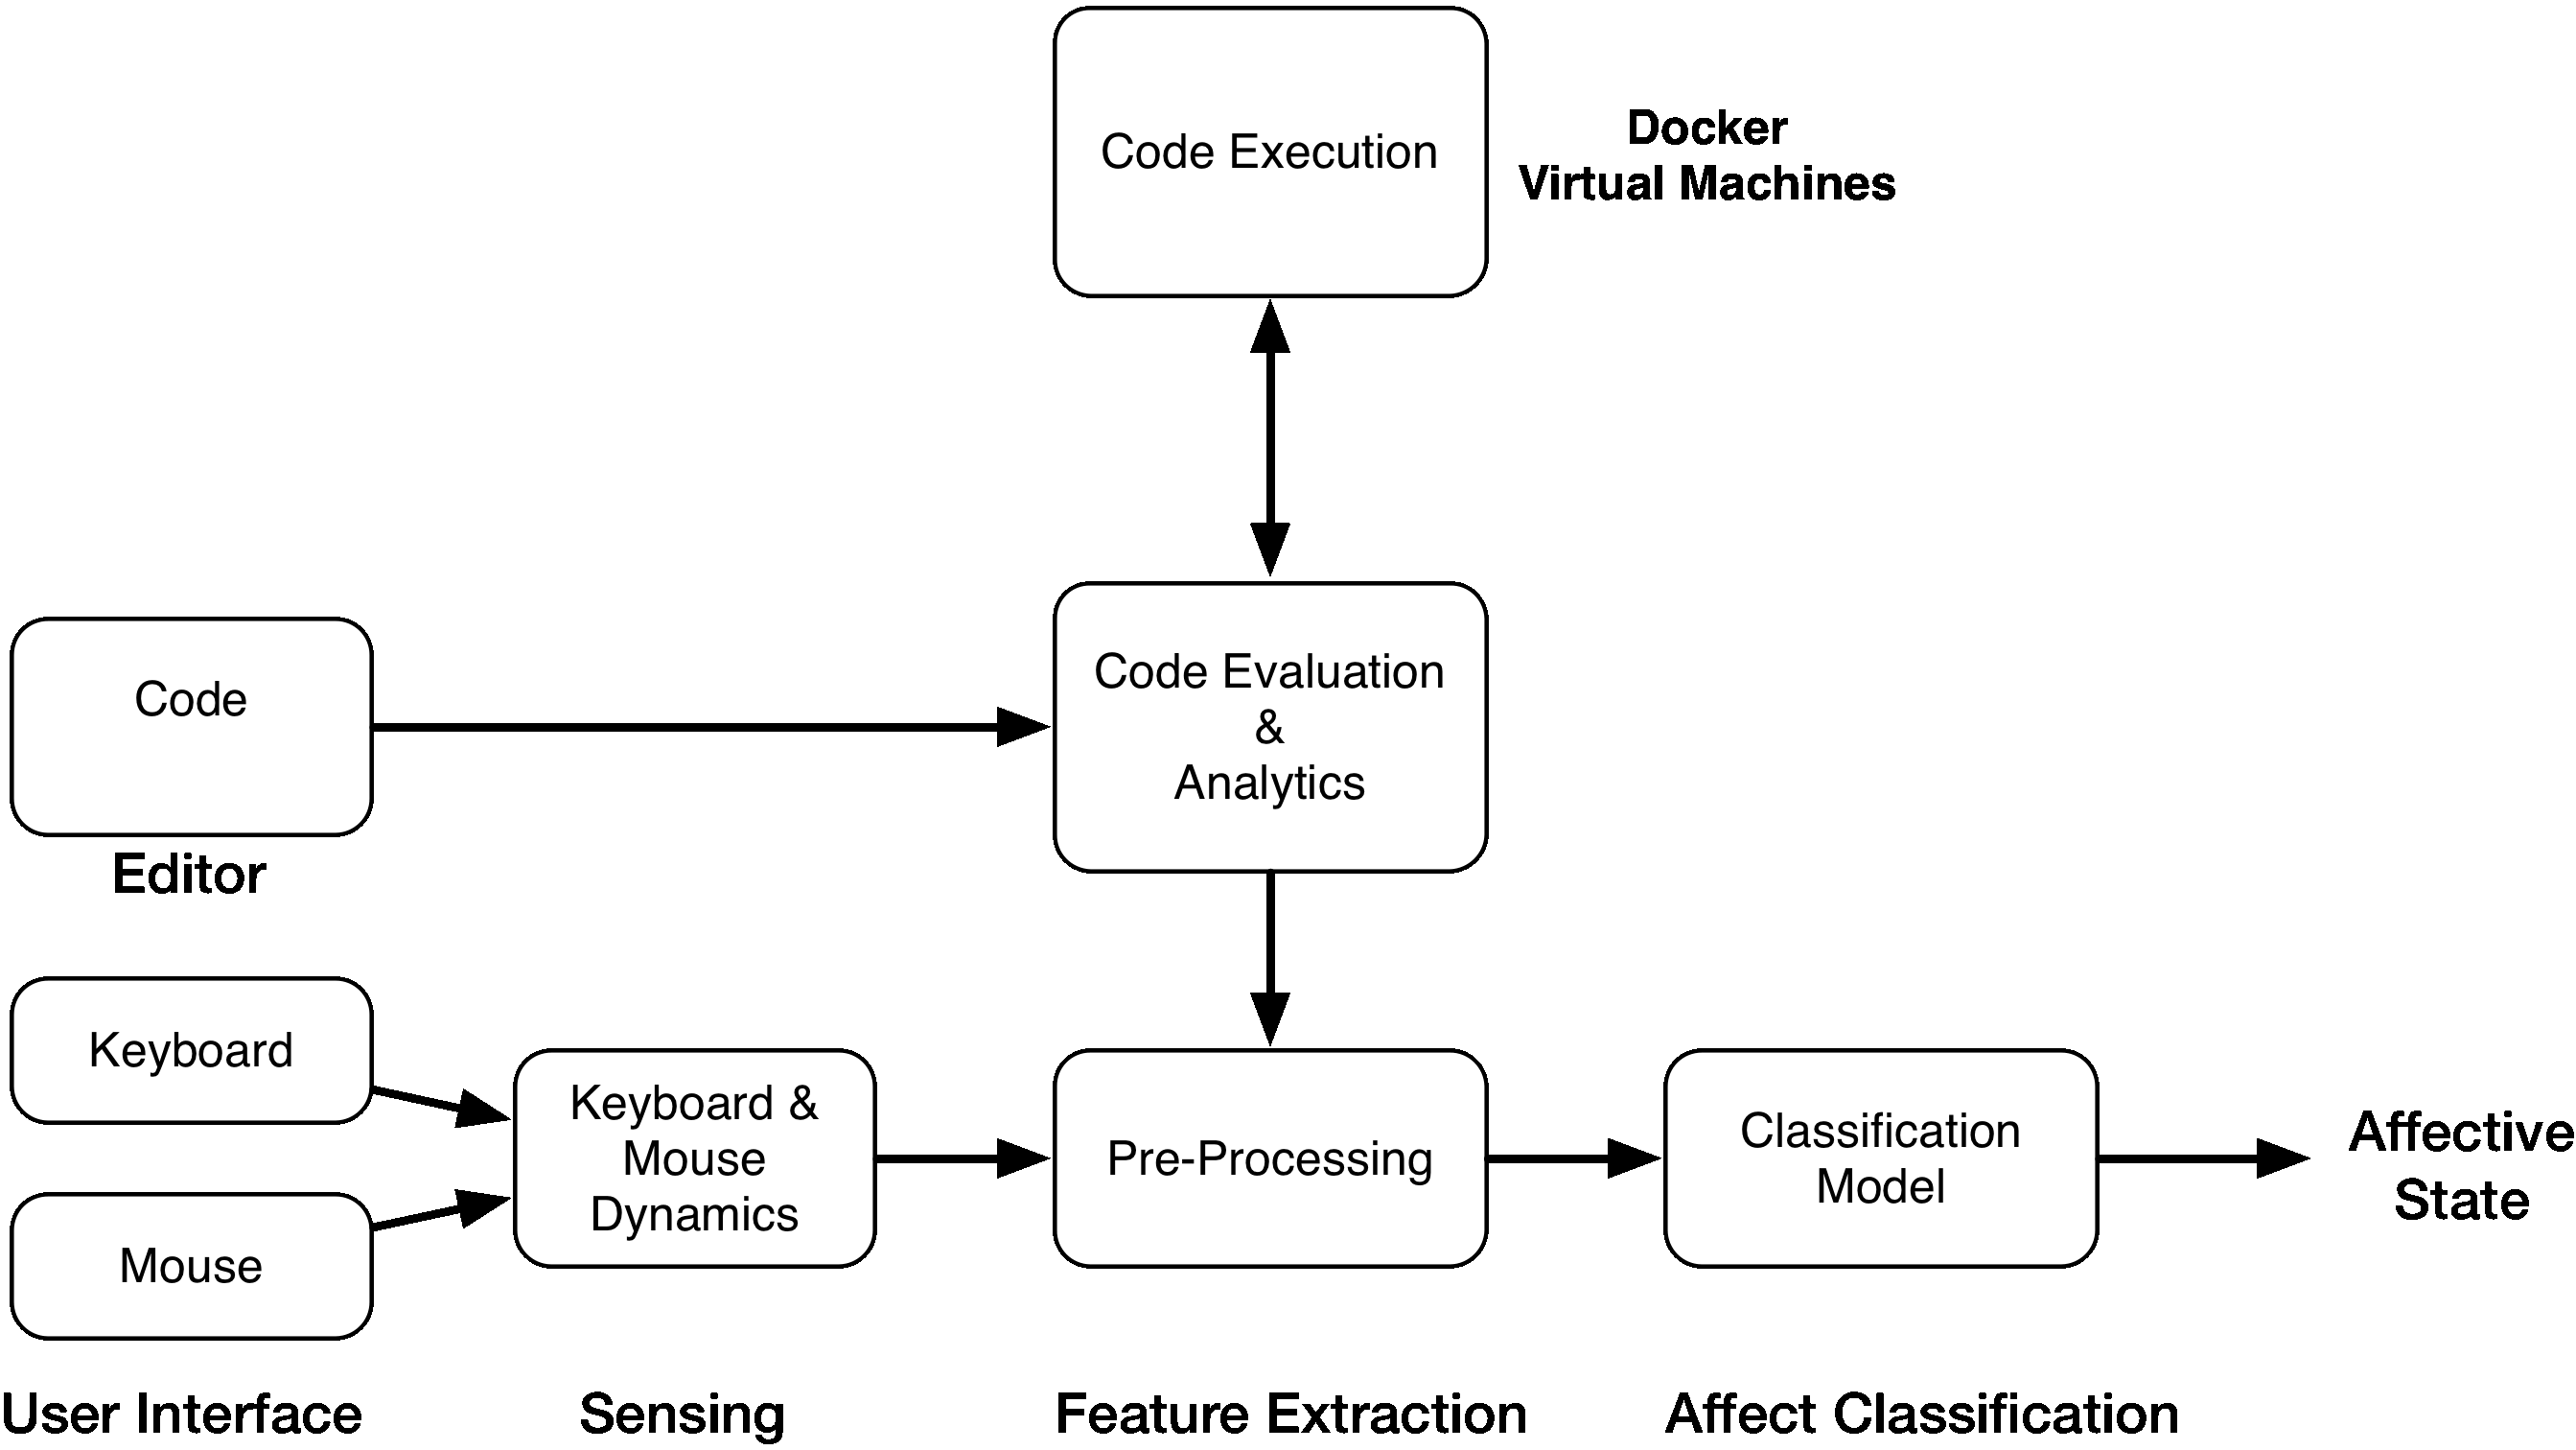
\includegraphics[width=2.5in]{KMD_Affective} 
% where an .eps filename suffix will be assumed under latex,  
% and a .pdf suffix will be assumed for pdflatex; or what has been declared 
% via \DeclareGraphicsExtensions. 
\caption{Simulation results for the network.}
\label{fig_sim} 
\end{figure}

% Note that the IEEE typically puts floats only at the top, even when this
% results in a large percentage of a column being occupied by floats.






% use section* for acknowledgment 
\section*{Acknowledgment} 
This received funding from Tecnólogico Nacional de México through the project: Técnicas de
computación inteligente para el secuenciado adaptativo de ejercicios de
programación en la nube.
  


% trigger a \newpage just before the given reference 
% number - used to balance the columns on the last page 
% adjust value as needed - may need to be readjusted if 
% the document is modified later %\IEEEtriggeratref{8} 
% The "triggered" command can be changed if desired:
%\IEEEtriggercmd{\enlargethispage{-5in}}

% references section

% can use a bibliography generated by BibTeX as a .bbl file 
% BibTeX documentation can be easily obtained at: 
% http://mirror.ctan.org/biblio/bibtex/contrib/doc/ 
% The IEEEtran BibTeX style support page is at: 
% http://www.michaelshell.org/tex/ieeetran/bibtex/
\bibliographystyle{IEEEtran} 
% argument is your BibTeX string definitions and bibliography database(s) 
\bibliography{programming} 
% 
% <OR> manually copy in the resultant .bbl file 
% set second argument of \begin to the number of references 
% (used to reserve space for the reference number labels box)



% that's all folks 
\end{document}


